\subsection*{Level 1}
\addcontentsline{toc}{subsection}{Level 1}

In this section, we need to design the linear friction $d_1$ in the friction model $M_f = d_1 \dot{\varphi}$ and the total inertia $J$.

The parameter identification is done using a step time $T_s = 10 \text{ ms}$.

In order to do so, we add our motor model to ControlDesk. We then fit the theoretical curve to the real one (using sliders to modify $d_1$ and $J$). 

The fitted curves for motor 1 and motor 2 are on Figure \ref{fittedCurves}. 

%---------------------------------------------
% WARNING: The real curves are oscillating, due to ????
%---------------------------------------------

We have the following values:

\begin{center}
\begin{tabular}{|c|c|c|}
 \hline
 & Motor 1 & Motor 2 \\
 \hline 
 $J$ & $4.2e-7$ & $4.6e-6$ \\ 
 \hline 
 $d_1$ & $4.8e-6$ & $5.8e-6$  \\
 \hline
\end{tabular}
\end{center}


\begin{center}
\begin{figure}[ht]
 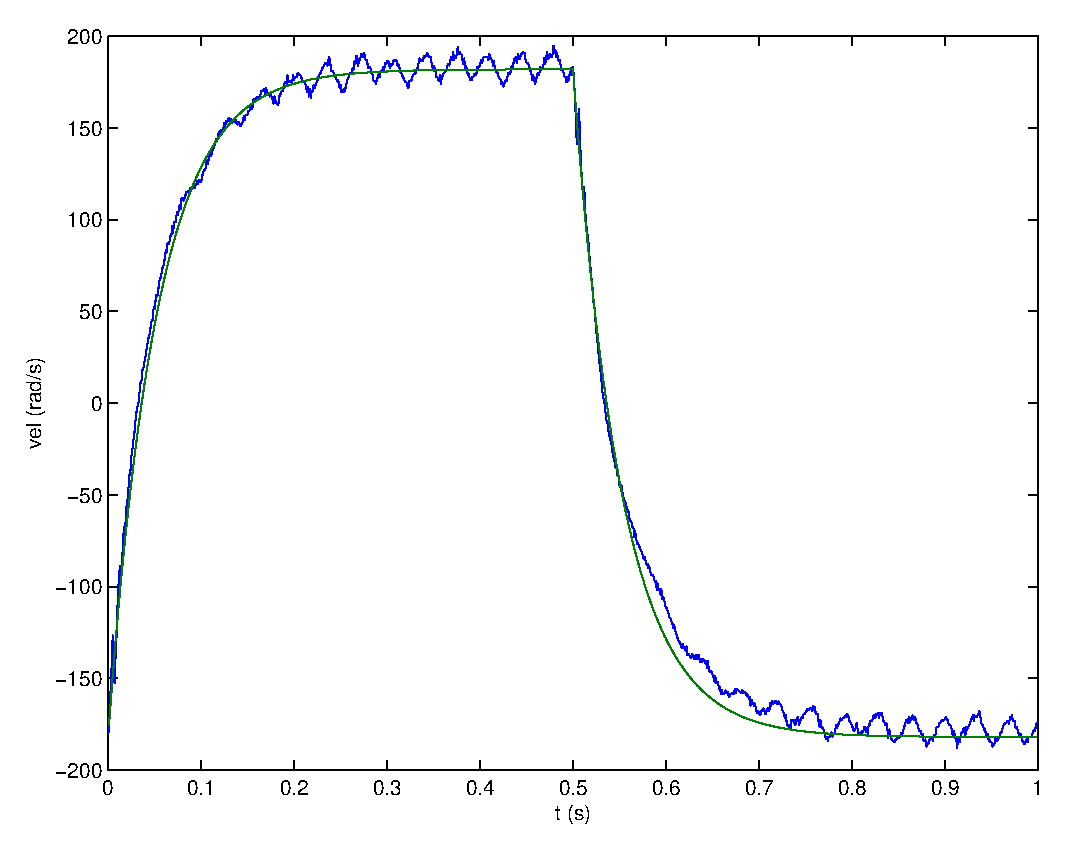
\includegraphics[width=\linewidth]{fig/motor1L1.eps}
 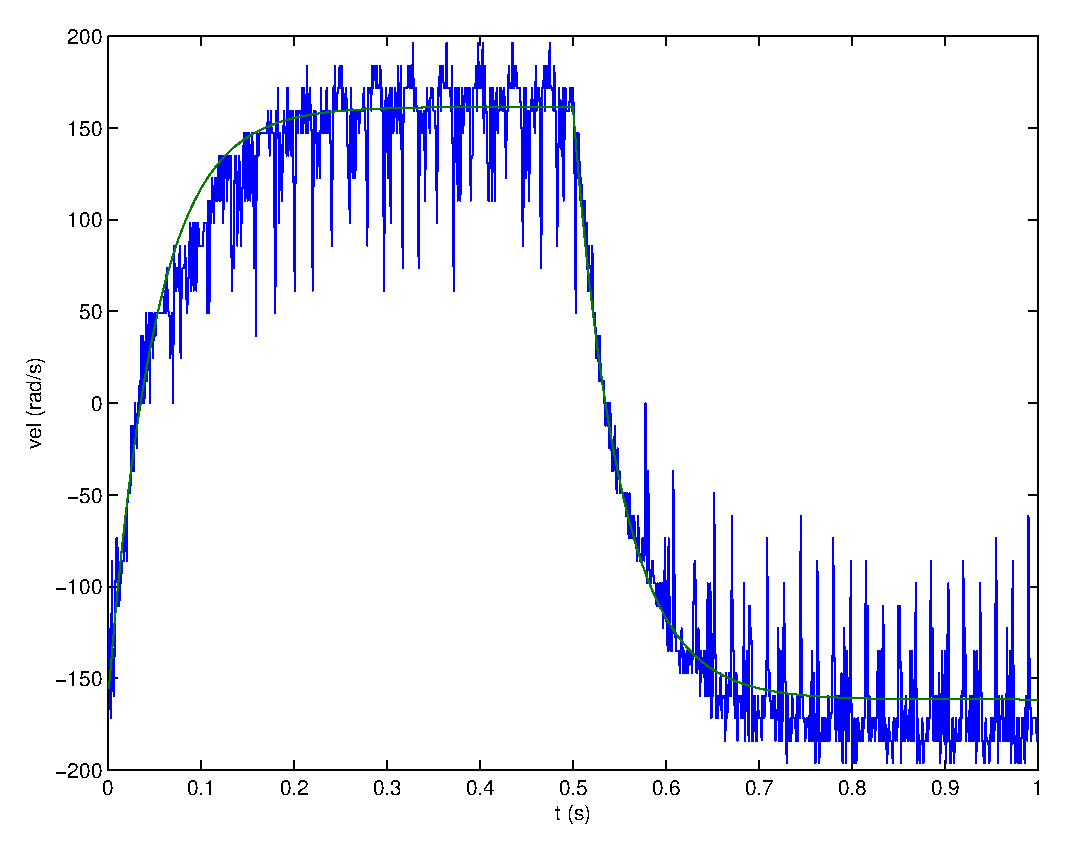
\includegraphics[width=\linewidth]{fig/motor2L1.eps}
 \caption{Fitted curves for motor 1 \& 2 -- green \\ Real curves for motor 1 \& 2 -- blue}
 \label{fittedCurves}
\end{figure}
\end{center}

\subsection*{Level 2}
\addcontentsline{toc}{subsection}{Level 2}

In this section, we identify the parameters for a second model with a nonlinear friction model $M_f = d_2 \varphi + F_c \sgn(\varphi)$, which includes static friction, using the Karnop friction model.

The parameter identification is done using a step time $T_s = 10 \text{ ms}$.

To do so, we add our motor model to ControlDesk. We the fit the theoretical curve to the real one (using sliders to modify $d_2$ and $F_c$).

The fitted curves for motor 1 and motor 2 are on Figure \ref{fittedCurves2} (from a two steps with different amplitudes). Figure \ref{sinFitted} shows the velocity signal with a sinewave input with low amplitude.

We have the following values:


\begin{center}
\begin{tabular}{|c|c|c|}
 \hline
 & Motor 1 & Motor 2 \\
 \hline 
 $d_2$ & $1.0e-8$ & $1.0e-8$ \\ 
 \hline 
 $F_c$ & $1.0e-4$ & $1.0e-4$  \\
 \hline
\end{tabular}
\end{center}

%---------------------------------------------
% WARNING: Missing analysis here
%---------------------------------------------

Considering the non linear friction model improve the quality of our model.

%---------------------------------------------
% WARNING: WRONG CURVES HERE
%---------------------------------------------
\begin{center}
\begin{figure}[ht]
 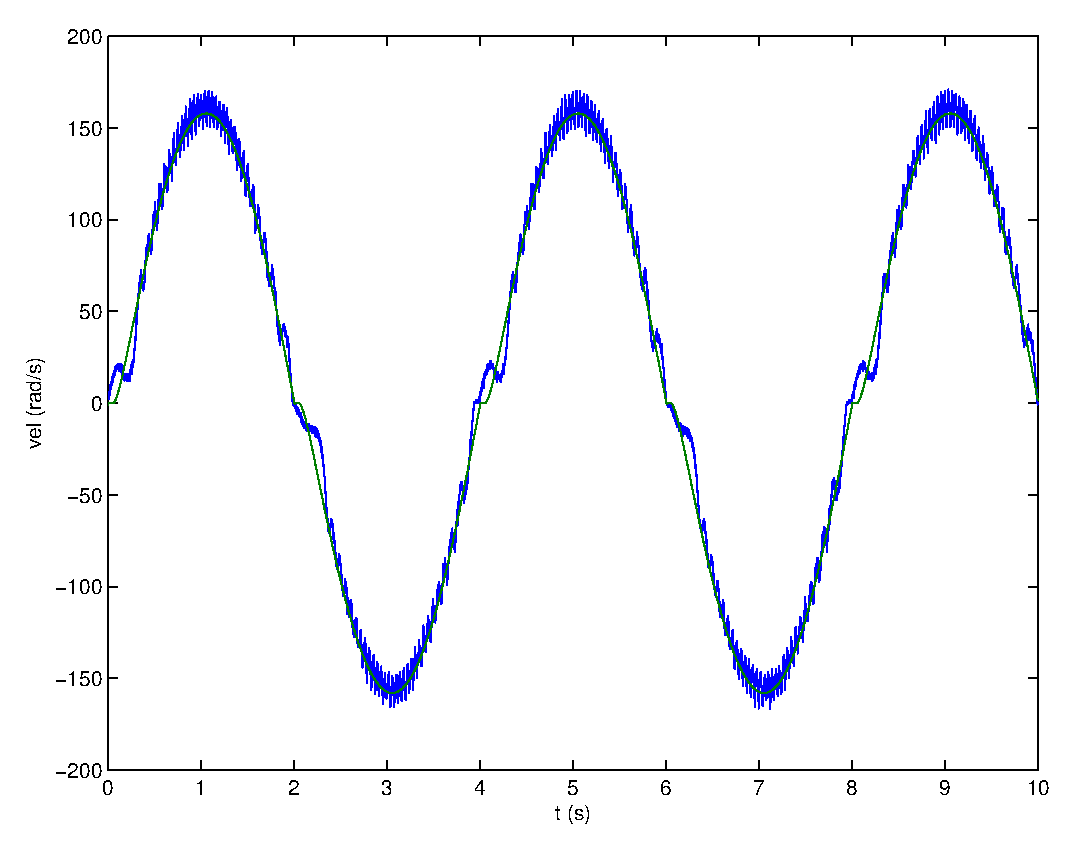
\includegraphics[width=\linewidth]{fig/motor1L2_2.eps}
 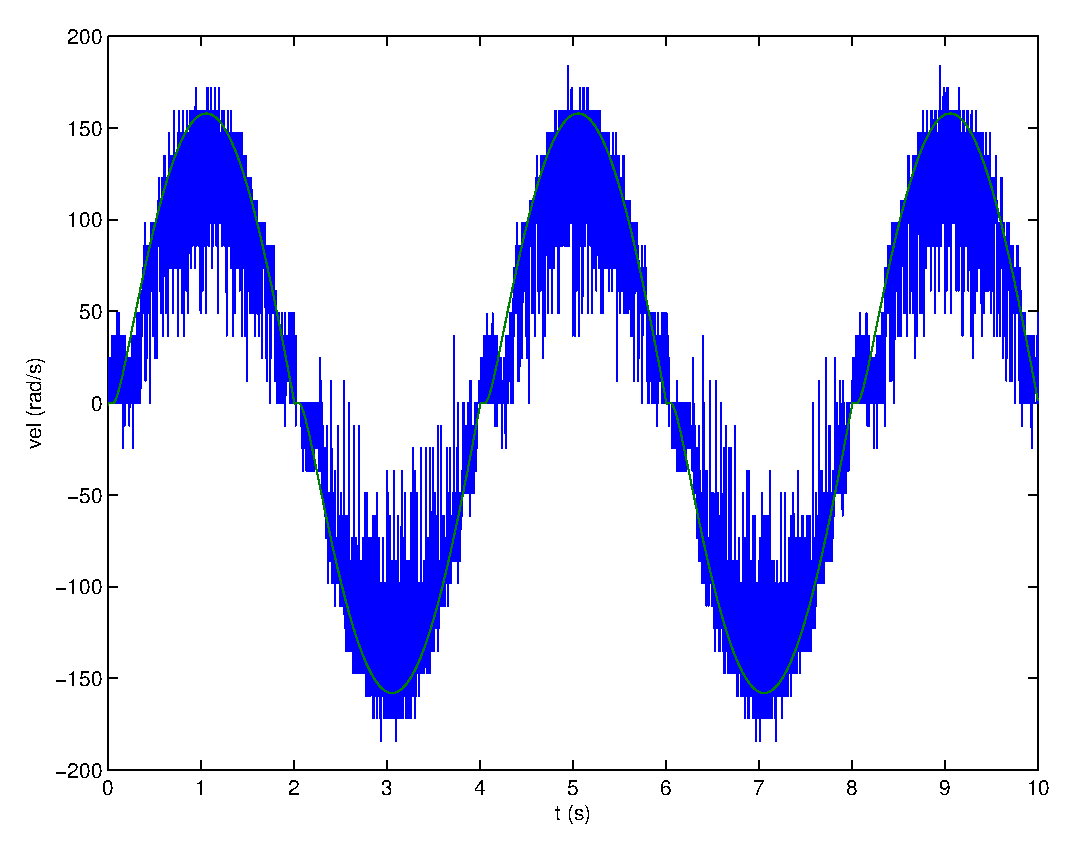
\includegraphics[width=\linewidth]{fig/motor2L2_2.eps}
 \caption{Fitted curves for motor 1 \& 2 -- green \\ Real curves for motor 1 \& 2 -- blue}
 \label{fittedCurves2}
\end{figure}
\end{center}

\begin{center}
\begin{figure}[ht]
 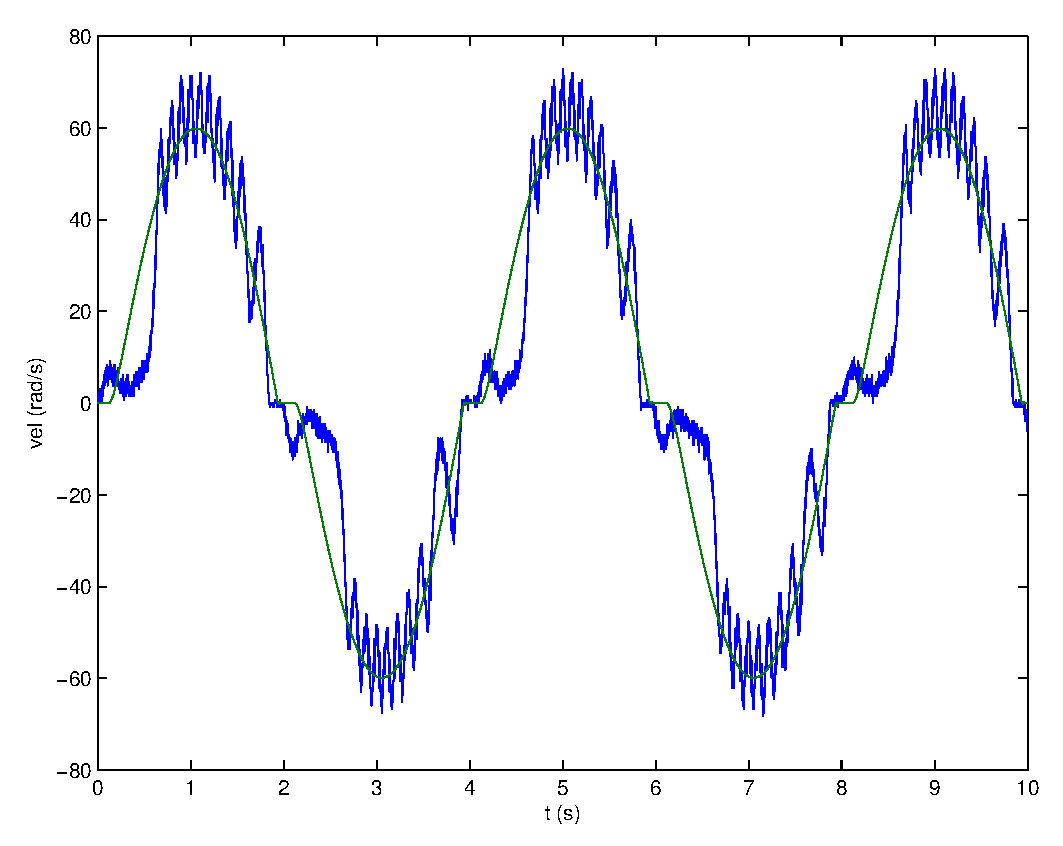
\includegraphics[width=\linewidth]{fig/motor1L2_1.eps}
 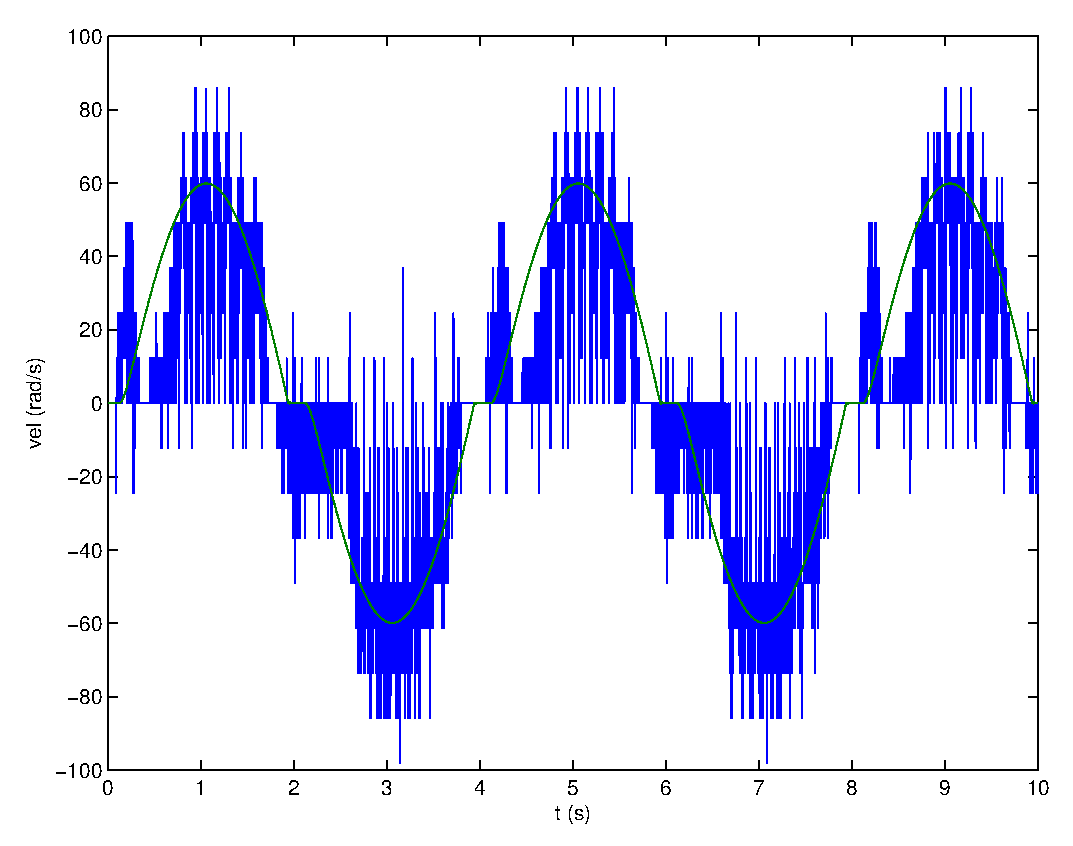
\includegraphics[width=\linewidth]{fig/motor2L2_1.eps}
 \caption{Motor response for a sinewave of low amplitude \\ Theoretical curves for motor 1 \& 2 -- green \\ Real curves for motor 1 \& 2 -- blue}
 \label{sinFitted}
\end{figure}
\end{center}

